\documentclass[runningheads]{llncs}
\usepackage[T1]{fontenc}
\usepackage{lmodern}
\usepackage{microtype}
\setlength{\emergencystretch}{1.5em}
\setlength{\textfloatsep}{13pt plus 3pt minus 2pt}
\setlength{\floatsep}{11pt plus 2pt minus 2pt}
\usepackage{graphicx,amsmath,amssymb,booktabs,tabularx,multirow,url}
\usepackage[hidelinks]{hyperref}
\hypersetup{pdftitle={EvidencePath: Analyzing Candidate Coverage and Ranking in Cross-Cancer Drug Retrieval},pdfauthor={Anonymous Authors}}
\graphicspath{{assets/}}
\newcommand{\Rzero}{R_0}
\newcommand{\Runion}{R_1}
\newcommand{\rr}{\operatorname{RR}}
% Set this to the verified anonymous repository URL to display it in Section 4.
\newcommand*{\artifacturl}{https://anonymous.4open.science/r/EvidencePath-A6E6/}
\begin{document}
\title{EvidencePath: Analyzing Candidate Coverage and Ranking in Cross-Cancer Drug Retrieval}
\titlerunning{EvidencePath: Candidate Coverage and Ranking}
\author{Anonymous Authors}
\authorrunning{Anonymous Authors}
\institute{}
\maketitle
\begin{abstract}
We investigate how partially overlapping PrimeKG and CIViC candidate lists affect retrieval of later qualifying CIViC annotations for retrospectively identified cancer--molecular-profile queries. EvidencePath combines frozen retrieval with diagnostics of candidate coverage, shared membership, and source ordering. On 45 replay queries with 46 positive pairs, standard reciprocal rank fusion (RRF) reaches query mean reciprocal rank (MRR) 0.3895, compared with 0.3460 for Context on the same union and 0.4265 for a parameter-free shared-first Context control; all three achieve HR@5 of 27/45. The observed RRF--Context difference does not establish a stable advantage in this sample. Frozen-score decomposition shows how wider coverage can be outweighed by displacement of previously reachable positives. Conditional order permutations, source-overlap sensitivity analysis, and an exact bound for merging two fixed sequences make these comparisons inspectable. Together, these post hoc diagnostics clarify how access, shared membership, and ordering relate to retrieval outcomes, revealing depth-dependent performance differences and trade-offs between finding evidence-exclusive positives and retaining earlier hits.
\keywords{Drug retrieval \and Heterogeneous evidence \and Rank fusion \and Knowledge graphs \and Temporal evaluation}
\end{abstract}
\section{Introduction}
\label{sec:intro}
Adding an evidence source changes both which candidates a query can retrieve and which appear near the top. For a joint cancer and molecular-profile query, PrimeKG supplies mechanism-linked drug candidates, while CIViC records evidence with disease, profile, direction, and provenance~\cite{primekg,civic2022}. Clinical evidence can recover a positive absent from the graph pool, but combining the pools also changes competition with previously reachable positives.

We study retrieval of \emph{later qualifying CIViC annotations}, rather than prediction of treatment efficacy. The main retrospective replay contains 45 cancer--profile queries and 46 positive drug pairs. Its query descriptors are identified from the endpoint, while candidate retrieval and ranking use each window's opening evidence snapshot. Three queries identifiable at the window start form a separate, smaller cohort. Thus later entry into the knowledgebase is the evaluation event; it need not represent a newly discovered biological association or a prospectively available query.

Partially overlapping candidate lists introduce a second distinction beyond coverage. A shared drug contributes a rank from each branch under standard reciprocal rank fusion (RRF)~\cite{rrf}. An observed gain may therefore be reproduced by a simple rule favoring shared membership, even without RRF's particular use of within-list ranks. We ask how candidate access, a shared-first control, and conditional changes to source order correspond to retrieval outcomes, and how those outcomes vary with retrieval depth. The comparisons diagnose fixed inputs; they do not causally partition biomedical information.

The replay illustrates why a strong same-pool comparison matters. RRF reaches query mean reciprocal rank (MRR) 0.3895 versus 0.3460 for Context, but paired 95\% cluster-bootstrap intervals under both drug- and source-defined query groups span zero. A parameter-free shared-first Context rule reaches 0.4265, and all three policies hit 27/45 queries in the top five. The observed ordering reverses in development: RRF reaches 0.4594 versus 0.3750 for shared-first Context. These results do not establish either policy as a general winner; they show that an RRF advantage over appending does not establish an advantage of its ranking rule over simpler same-union controls.

Access and placement also differ under frozen scoring. In replay, expansion raises pair coverage from 20/46 to 33/46, while rescoring lowers MRR from 0.1902 to 0.1809. The gain from newly reachable positives is smaller than the displacement loss on original positives. EvidencePath preserves canonical single-drug identity, branch membership, ranks, and provenance to make these comparisons inspectable. SF includes both graph features and drug-level CIViC counts; the graph pool is not a pure graph-feature baseline. All added controls are post hoc diagnostics on exposed cohorts, with frozen models and fusion defaults.

We make three contributions.
\begin{enumerate}
\item \textbf{A traceable retrospective retrieval setting.} We separate development, cutoff-defined queries, and endpoint-defined replay, retain complete positive denominators, and connect frozen candidate lists to their visible evidence and later annotation sources.
\item \textbf{Fixed-pool diagnostics of coverage, membership, and ordering.} An MRR decomposition, paired cluster analyses, and a shared-first control test whether observed fusion gains persist against competitive same-union alternatives, while retaining uncertain and unfavorable outcomes.
\item \textbf{Evidence on depth-dependent trade-offs and conditional limits.} Source-order permutations, new-positive versus old-hit retention, source-overlap sensitivity, and an exact two-sequence ceiling characterize what the measured policies achieve under specified inputs and constraints.
\end{enumerate}

\section{Related Work}
\label{sec:related}
\paragraph{Drug retrieval over heterogeneous evidence.}
Drug repurposing links mechanisms to potential therapeutic uses~\cite{pushpakom}. PrimeKG provides a biomedical graph~\cite{primekg}; TxGNN predicts disease-level indications and contraindications~\cite{txgnn}, and AURORA scores drug--disease associations~\cite{aurora}. PanDrugs2 prioritizes therapies from individual multi-omics inputs~\cite{pandrugs2}. Their inputs and endpoints differ from later annotation retrieval for a cancer--profile key, so their task-level scores are not matched comparisons here.

\paragraph{Clinical knowledge and gene--drug retrieval.}
CIViC retains direction, level, and provenance for profiles that may contain multiple variants~\cite{civic,civic2022,civiccuration,civicmp}. OncoKB and ESCAT organize contextual actionability~\cite{oncokb,escat}. GeneDrug retrieves gene--drug evidence, while GGEF evaluates relation extraction from cancer guidelines~\cite{genedrug,ggef}. We hold evidence visibility and candidate construction fixed when comparing the ordering of canonical drugs.

\paragraph{Learning to rank and fusion.}
We use LambdaMART with LightGBM and metasearch aggregation~\cite{lambdamart,lightgbm,metasearch,rrf}. Bruch et al.\ compare score convex combinations with RRF and examine parameter sensitivity~\cite{bruch}. Exp4Fuse combines original- and LLM-expanded-query routes and weights fusion using the number of lists containing a document~\cite{exp4fuse}. Shared support is therefore an existing fusion signal. We use standard RRF and diagnose fixed biomedical lists; we claim neither a new fusion rule nor superiority over untested rules.

\paragraph{Evaluation with evolving knowledge.}
Retrospective estimates depend on query selection, information visibility, and model-selection exposure~\cite{cawley,kapoor}. Dated exports make these boundaries inspectable but do not create an independent prospective validation. Sect.~\ref{sec:eval} separates the evaluation populations and specifies the paired, conditional, and provenance-based analyses.

\section{Task and EvidencePath Design}
\label{sec:method}
\subsection{Query, candidate, and target semantics}
A query $q=(c,m)$ pairs a cancer label with a CIViC molecular profile (MP) identifier. Frozen normalization defines each single drug $d$. Records retain evidence-item and source identifiers but contribute one $(q,d)$ evaluation pair. Distinct profiles remain distinct targets.

Graph pool $R_0(q)$ and evidence pool $E(q)$ give lists $L_g(q)$ and $L_e(q)$. Their union is $R_1(q)=R_0(q)\cup E(q)$, with additions $N(q)=E(q)\setminus R_0(q)$ and shared members $S(q)=R_0(q)\cap E(q)$. An empty graph branch does not remove a query from evaluation.

The endpoint set $P(q)$ includes all eligible positives, including drugs outside $R_1$. A therapy and blank-interaction screen precedes frozen single-drug adjudication, excluding generic classes and combinations. Positives require accepted predictive evidence supporting sensitivity/response at level A--D. We exclude pairs with both A/B support for sensitivity/response and A/B support for resistance or non-support for sensitivity/response. This eligibility rule is independent of the ranking conflict flag. Targets are annotations, not patient treatment outcomes.

\subsection{Source orders and membership control}
Figure~\ref{fig:framework} outlines the workflow. D1--D4 and ranks are illustrative; \emph{new} denotes evidence-exclusive candidates relative to $R_0$, and recall denotes positive-pair coverage.
\begin{figure}[t]
\centering
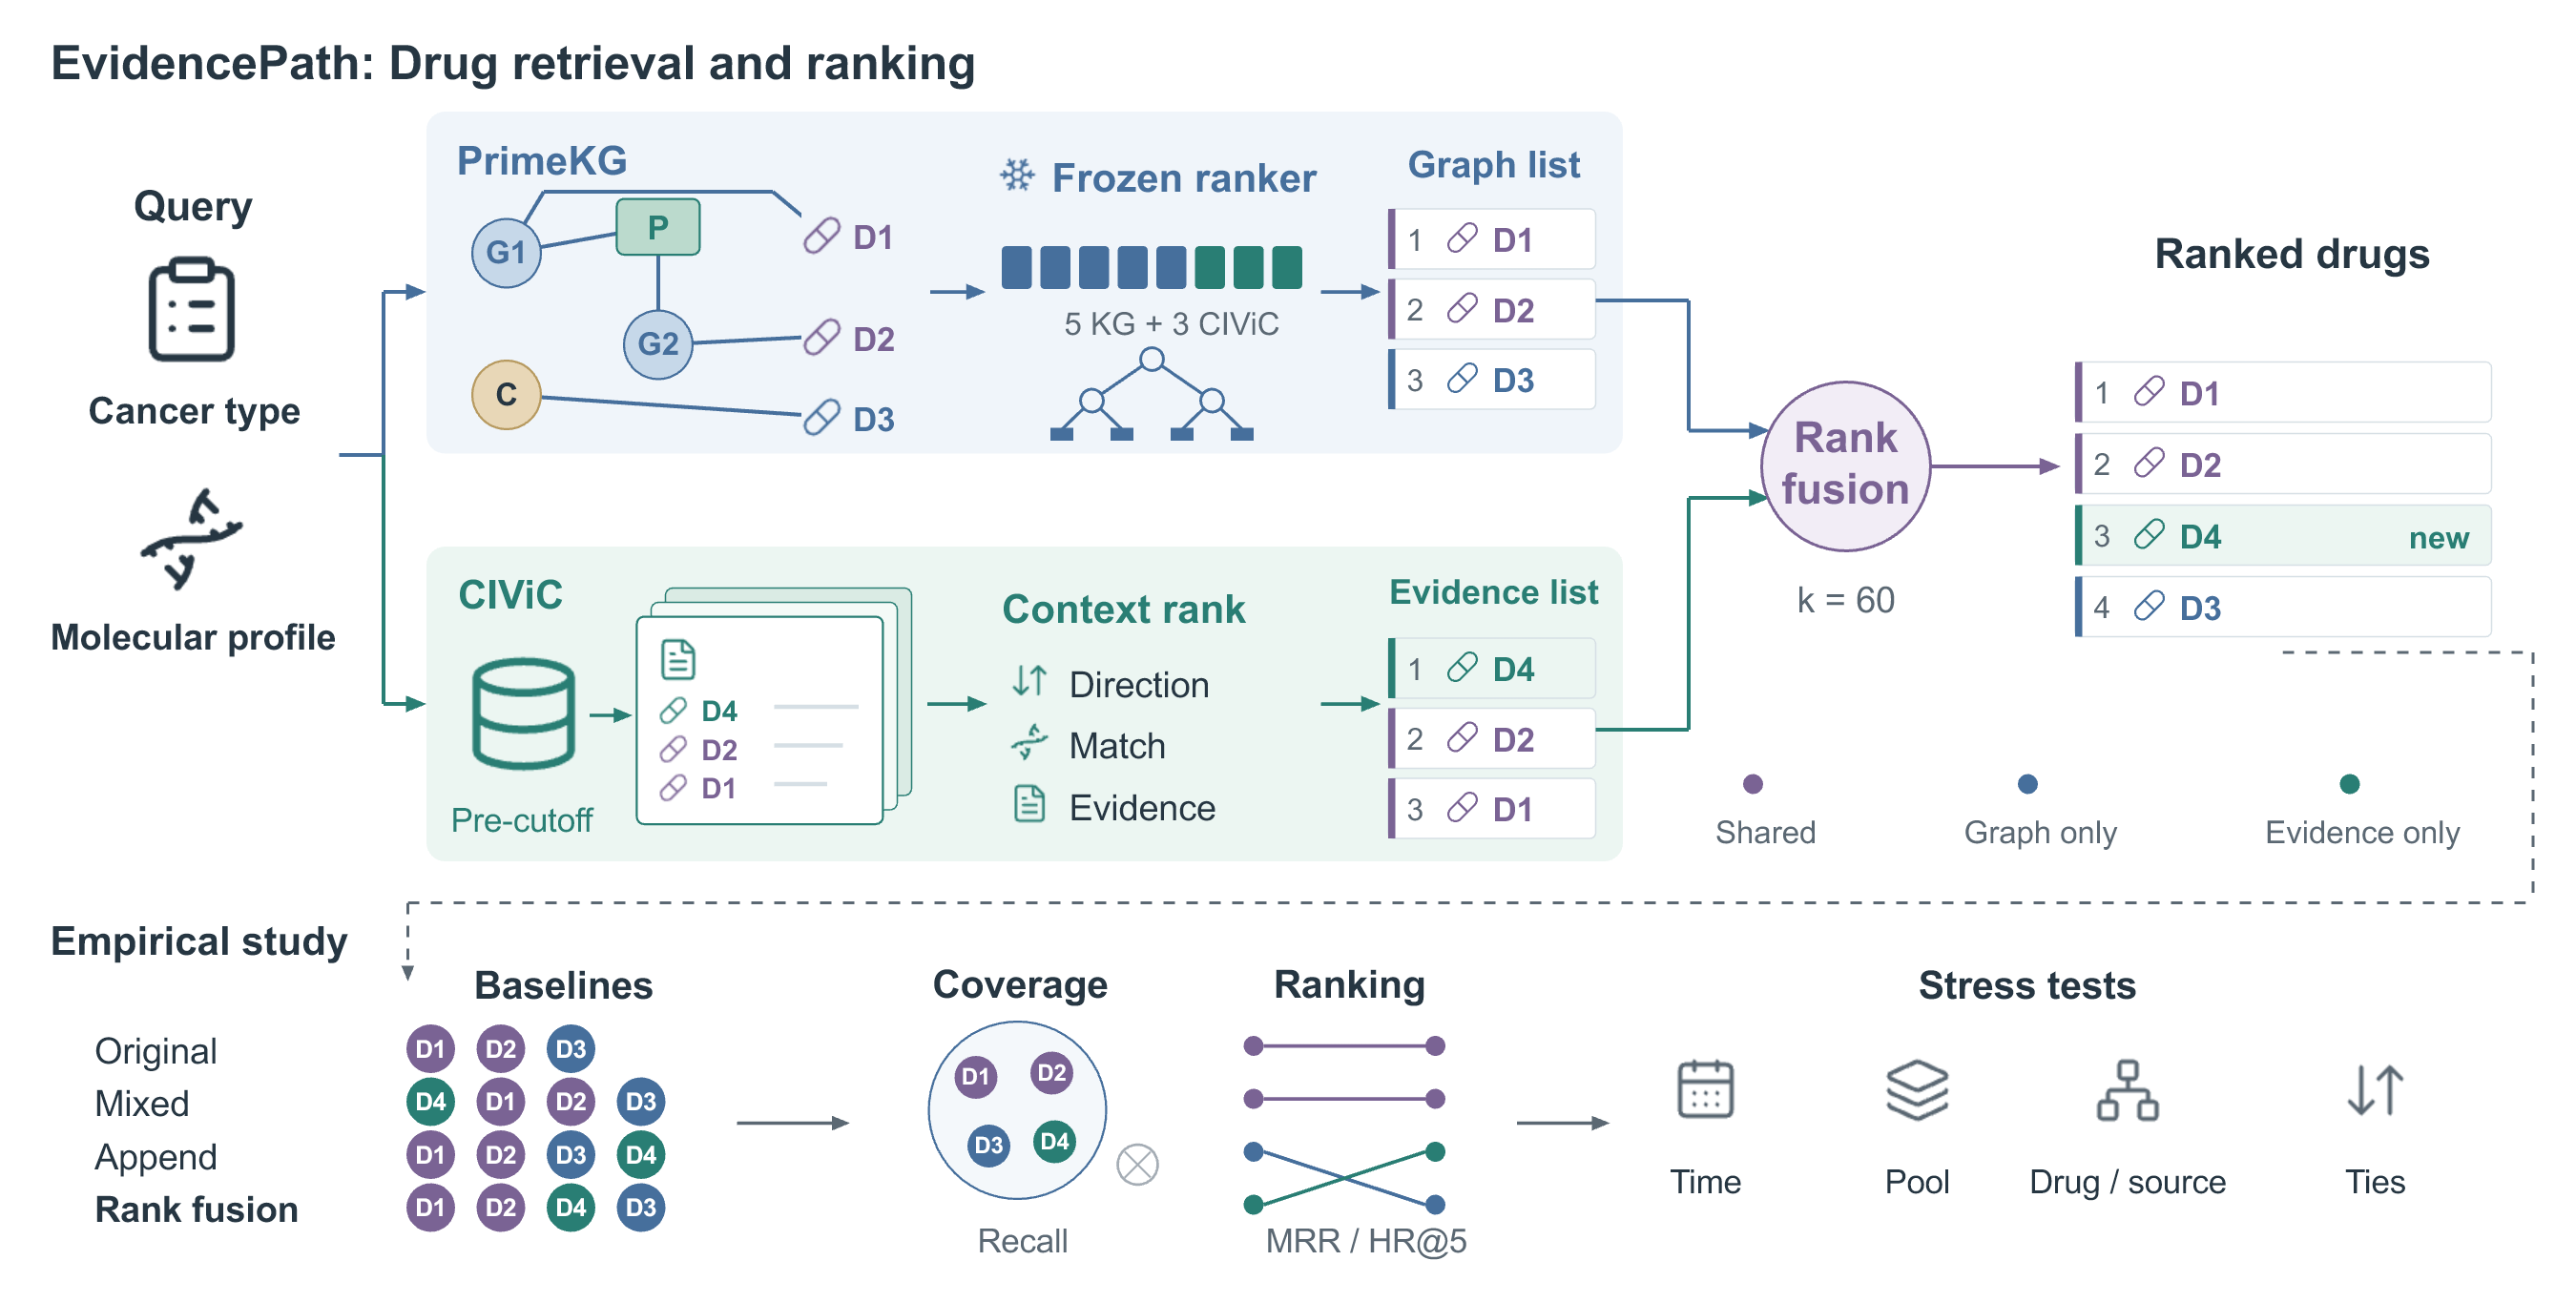
\includegraphics[width=\textwidth]{evidencepath-framework.png}
\caption{Workflow}
\label{fig:framework}
\end{figure}
\paragraph{Graph retrieval and frozen scoring.}
The graph branch unions direct targets, indications, and top-30 shared-pathway candidates (Table~\ref{tab:settings}).

SF is a frozen LightGBM LambdaMART ranker using graph and drug-level CIViC evidence (Table~\ref{tab:settings}). It scores the union once. The graph list restricts those scores to $R_0$, sorting by decreasing score then ascending canonical name. Graph names a pool, not a graph-feature-only scorer.

\paragraph{Clinical retrieval and order.}
Cutoff CIViC retrieval links identical profiles or shared validated genes in accepted predictive single-drug records, without an additional list truncation. Support for sensitivity/response is benefit; support for resistance, reduced sensitivity or adverse response is adversity. Non-support for sensitivity/response is anti-benefit. Other combinations are undetermined.

The descending key $(b,m,c,h,\ell,n,f)$ precedes ascending name. Benefit sets $b=2$, only opposition sets $b=0$, otherwise $b=1$. In tier 2, the best benefit maximizes $(m,c,\ell)$. Profile rank $m$ is 2 for identity or 1 for a shared gene. Disease rank $c$ is 2 for normalized equality, 1 for another known disease, or 0 for generic/missing disease. Levels A--E map to 5--1. Conflict sets $h=0$ if opposition has profile rank at least $m$, regardless of disease or level, otherwise $h=1$; the tier remains intact. Distinct benefit sources give $n$, SF gives $f$, and unused fields are zero. In tier 0, $\ell$ is the negative level of opposition selected by $(m,c,\ell)$.

\paragraph{Aggregation and control.}
For one-based source ranks, standard RRF is
\begin{equation}
s_{\mathrm{RRF}}(q,d)=\sum_{b\in\{g,e\}:\,d\in L_b(q)}\frac{1}{k+r_b(q,d)},\qquad k=60.
\label{eq:rrf}
\end{equation}
Each present branch contributes one equal-weight term. We compare rational scores exactly and break ties by name. Shared members receive two terms, exclusive members one. Length-normalized Borda sums $(|L_b|-r_b+1)/|L_b|$ over present lists and assigns zero for absence, using double precision and the same final tie rule. Aslam and Montague distribute remaining points to unranked items~\cite{metasearch}.

Context applies the full key to $R_1$. The parameter-free \emph{Shared-first} control stably places $S(q)$ before $R_1(q)\setminus S(q)$ in that full Context order. It preserves candidates, labels and within-block Context order, and is a post hoc diagnostic, not a validated new default.

\subsection{Separating coverage from displacement}
\label{sec:decomposition}
Let $\rr_M(q,d)=1/r_M(q,d)$ for a retrieved drug and zero otherwise, and $u_M(q)=\max_{d\in P(q)}\rr_M(q,d)$. Graph ranks $R_0$ and Mix ranks $R_1$ using the same frozen scores. Append-SF concatenates $O=L_g$ with SF-ordered additions $N_{\mathrm{SF}}$. Define $u_{\mathrm{Mix},0}$ at full Mix positions, maximizing only over $P(q)\cap R_0(q)$, or zero for an empty set. Then
\begin{align}
u_{\mathrm{Mix}}(q)-u_{\mathrm{Graph}}(q)
={}&\underbrace{u_{\mathrm{Mix},0}(q)-u_{\mathrm{Graph}}(q)}_{\text{original-positive displacement}}\nonumber\\
&+\underbrace{u_{\mathrm{Mix}}(q)-u_{\mathrm{Mix},0}(q)}_{\text{newly accessible-positive increment}}.
\label{eq:decomposition}
\end{align}
Both means use the same queries. With unchanged original scores and ties, Mix keeps the relative $R_0$ order, so the first term is nonpositive; the second is nonnegative. Append-SF fixes original absolute positions. We check these conditions against scores and historical exports.

\subsection{A limit of merging two fixed sequences}
\label{sec:bound}
Aslam and Montague's oracle follows unanimous pairwise preferences~\cite{metasearch}. Our conditional oracle preserves every within-list precedence of disjoint $O$ and $N_e$, the evidence-exclusive additions in $L_e$ order. If their first positive positions are $i^*,j^*$, or infinity when absent, the best merge attains
\begin{equation}
u_{\mathrm{2seq}}^*(q)=\max\left\{\frac{1}{i^*(q)},\frac{1}{j^*(q)}\right\},\qquad 1/\infty=0.
\label{eq:bound}
\end{equation}
Each positive follows its within-sequence predecessors; placing the sequence with the earlier first positive first attains the bound. Averaging bounds merges of these specified sequences. An old-order oracle fixes only $O$ and frees additions. Exceeding the two-sequence bound requires relaxing at least one constraint, not necessarily the graph order.

\section{Experimental Protocol}
\label{sec:eval}
\ifx\artifacturl\empty\else
The archived baseline package is linked at the \href{\artifacturl}{anonymous artifact site}. Revision-specific outputs, evidence ledgers and generation commands accompany this version.
\par
\fi
\subsection{Snapshots and populations}
PrimeKG and both July-2025-supervised rankers stay frozen. January development uses July 2025 inputs and January 2026 labels; its 43 positive pairs include 40 first observations and three augmentations (Table~\ref{tab:datasets}).

\begin{table}[t]
\caption{Evaluation sets}
\label{tab:datasets}
\centering\small
\setlength{\tabcolsep}{4pt}
\begin{tabular}{@{}lrrl@{}}
\toprule
Population & Queries & Pairs & Role \\
\midrule
January development & 41 & 43 & Exposed development \\
Quarterly cutoff-defined & 3 & 3 & First observations \\
New-context replay & 45 & 46 & Main retrospective replay \\
Quarterly combined & 48 & 49 & Descriptive total \\
Quarterly augmentation & 1 & 1 & Separate secondary endpoint \\
\bottomrule
\end{tabular}
\end{table}

Quarterly windows run January--April, April--July and July--October 2026, using opening exports for inputs and closing exports for labels. First observations require an eligible positive with no earlier positive, first-observation assignment or eligible cutoff record. Other eligible events are augmentations; mapping-only changes are excluded.

Cutoff-defined keys have a predictive record with a therapy and blank interaction at opening, before drug qualification. New-context replay, defined retrospectively after the pilot, instead uses endpoint disease and profile descriptors for keys absent from that cutoff set. Retrieval and scoring still use cutoff evidence; endpoint drug and response supply labels. This is newly catalogued annotation retrieval, not prospective discovery. All 49 combined first observations cite literature from 2007--2025. January and quarterly labels share no canonical query or pair keys, which alone does not establish source independence.

\subsection{Fixed policies and settings}
\begin{table}[t]
\caption{Baselines}
\label{tab:baselines}
\centering\small
\setlength{\tabcolsep}{4pt}
\begin{tabularx}{\textwidth}{@{}llX@{}}
\toprule
Policy & Pool & Rule \\
\midrule
Graph & $R_0$ & Frozen SF order \\
Mix & $R_1$ & The same SF scores on the union \\
Append-SF & $R_1$ & $O$ then $N_{\mathrm{SF}}$ \\
AltGraph & $R_0$ & Frozen alternative order \\
AltAppend & $R_1$ & AltGraph then SF-ordered additions \\
Context & $R_1$ & Full context key on the union \\
Shared-first & $R_1$ & Shared block first; Context within blocks \\
CIViC & $E$ & Full clinical list with SF tie-break \\
Borda / RRF & $R_1$ & Aggregation of the same source lists \\
\bottomrule
\end{tabularx}
\end{table}
RRF minus Context is the primary same-pool contrast; RRF minus CIViC is secondary and uses different support. Context, Shared-first and RRF give two consecutive same-union changes. Graph versus Append-SF isolates additional access at fixed old positions; Eq.~\ref{eq:decomposition} diagnoses Mix versus Graph.

\begin{table}[t]
\caption{Frozen settings}
\label{tab:settings}
\centering\small
\setlength{\tabcolsep}{4pt}
\begin{tabularx}{\textwidth}{@{}lX@{}}
\toprule
Setting & Definition \\
\midrule
Five KG features & Direct target; $\log(1+\mathrm{shared\ pathways})$; profile-pathway coverage; Jaccard; indication \\
Three CIViC features & $\log(1+\mathrm{count})$ at A/B, C, D/E for visible drug evidence, pooled across contexts and directions \\
SF & 8D LambdaMART; 4 trees; rate .05; 7 leaves; depth $\leq3$; minimum leaf 3; L2=1; seed 7147 \\
AltGraph & 9D ordinal GBDT with graph-missing indicator; 2 trees; rate .05; seed 7147 \\
Supervision & 84 train pairs / 31 queries; 16 validation pairs / 7 queries; disjoint profiles \\
Retrieval cap & Shared pathways $\geq5$ and Jaccard $\geq0.08$; sort by decreasing Jaccard, decreasing profile-pathway coverage, then ascending name. Take Top-30 in this channel, then union with direct targets and indications. No extra cap on $E$ or $R_1$ \\
Rank fusion & RRF: $k=60$, equal branch weights \\
Insertion & Fixed $O$ and $N_v$ or $N_e$; $\lambda=4$ selected on development \\
\bottomrule
\end{tabularx}
\end{table}

For training \emph{and validation}, each candidate's registered label-defining EID union is excluded from its visible evidence. This exclusion is candidate-specific rather than publication-wide; unlabelled relevance remains unknown.

\begin{samepage}
\paragraph{Constrained insertion.}
Both policies preserve $O=(o_i)$ and additions $N'=(n_j)$. Original insertion uses $N_v$, sorted by priority $v$, SF score and then name; evidence insertion uses $N_e$. Priority is $(a-1)/(|R_1|-1)$, with $a$ the weak-to-strong average rank of $(b,m,c,h,\ell,n)$ over $R_1$. Use SF rank instead when $b<2,n=0$, and $v=1$ for singletons. With $D(r)=1/\log_2(1+r)$ and $s=|O|$, dynamic programming maximizes
\[
\begin{aligned}
&\sum_j v(n_j)\bigl[D(r_L(n_j))-D(s+j)\bigr] \\
&\quad-\lambda\sum_i D(i)\bigl[D(i)-D(r_L(o_i))\bigr].
\end{aligned}
\]
\end{samepage}

\subsection{Metrics and diagnostic procedures}
\label{sec:implementation}
All positives remain in the denominator, with RR zero when unretrieved. For queries $Q$ containing eligible positives,
\begin{align}
\mathrm{MRR}_{q}(M)&=\frac{1}{|Q|}\sum_{q\in Q}\max_{d\in P(q)}\rr_M(q,d),\label{eq:mrr}\\
\mathrm{MRR}_{p}(M)&=\frac{\sum_{q\in Q}\sum_{d\in P(q)}\rr_M(q,d)}{\sum_{q\in Q}|P(q)|}.\label{eq:pair}
\end{align}
HR@$K$ counts queries with a positive by rank $K$; coverage counts positive pairs in the pool. Replay query keys include the window.

\paragraph{Paired dependence checks.}
For replay we report paired RR differences and query-best-rank wins/ties/losses (W/T/L), with connected components under shared positive drugs or shared canonical positive-label sources. Partitions include transitive and cross-window links. Drug/source partitions contain 19/24 components, with largest sizes seven/six queries. Each of 10,000 PCG64 draws samples $C$ whole components with replacement. The statistic divides the summed paired differences by the \emph{actual sampled query count}, not by $C$. We report paired 95\% percentile intervals and leave-one-component analyses.

\paragraph{Conditional order permutations.}
We reuse archived 5,000-draw CIViC permutations and add 5,000 graph-order draws per cohort. Only selected within-query ranks are uniformly permuted; memberships, labels, the other branch's complete order, RRF parameters, per-candidate contribution counts and final tie rule stay fixed. Upper-tail counts use $T_{\rm perm}\geq T_{\rm obs}$ and $p=(b+1)/5001$. Holm correction covers 12 comparisons: two branches, two cohorts and MRR/HR@3/HR@5. Central 95\% ranges describe perturbations, not intervals for a method difference. Since CIViC retains SF, graph permutation tests additional graph order conditional on that list.

\paragraph{Shared-source label sensitivity.}
$I(q)$ unions IDs from cutoff evidence actually used for clinical retrieval/ordering or any candidate's SF counts, including opposing records. $L(q,d)$ contains all eligible supporting sources of a frozen positive. Normalize PubMed IDs and type other IDs; mark $I(q)\cap L(q,d)\ne\emptyset$ once, independently of hits. Remove overlapping labels only, keep ranks fixed, and drop queries without remaining positives. We report missing IDs and retained denominators. This differs from source occurrence anywhere in an opening export. All added diagnostics are post hoc; fixed settings do not make the exposed replay prospective.

\section{Results and Analysis}
\label{sec:results}
\subsection{Candidate access and displacement}
Table~\ref{tab:coverage} counts query--drug candidate records and covered positive pairs in both cohorts. The union expands positive access, but most graph candidates are not evidence members. In replay, shared membership accounts for only 120/1,580 candidate records yet contains 19/33 covered positives. The 318 evidence-exclusive records add 13 positives; the 1,142 graph-exclusive records add one.
% Generated from frozen artifacts; edit build_revision_tables.py, not numeric cells.
\begin{table}[t]
\centering
\caption{Candidate coverage}
\label{tab:coverage}
\small
\setlength{\tabcolsep}{4pt}
\begin{tabular}{lrrrr}
\toprule
Support & Dev. records & Dev. pairs & Replay records & Replay pairs \\
\midrule
Graph $R_0$ & 874 & 19/43 & 1,262 & 20/46 \\
Evidence $E$ & 360 & 23/43 & 438 & 32/46 \\
Union $R_1$ & 1,051 & 24/43 & 1,580 & 33/46 \\
Shared $R_0\cap E$ & 183 & 18/43 & 120 & 19/46 \\
Graph only & 691 & 1/43 & 1,142 & 1/46 \\
Evidence only & 177 & 5/43 & 318 & 13/46 \\
\bottomrule
\end{tabular}
\end{table}


Wider access does not ensure better placement. Replay Mix loses 0.0093 query MRR relative to Graph despite raising pair coverage from 20/46 to 33/46. Equation~\eqref{eq:decomposition} attributes this change to original-positive displacement of $-0.0310$ and a newly accessible-positive increment of $+0.0217$. The same SF scores are used before and after expansion. Thus displacement reflects insertion of additions ahead of old positives, not model refitting or a score change.

Development shows the same distinction at a larger magnitude: Mix loses 0.0641 MRR, comprising $-0.1395$ displacement and $+0.0754$ access gain. Append-SF fixes old absolute positions and gains 0.0737 over Graph. Its replay gain is smaller, $+0.0102$ (Table~\ref{tab:main}).

\subsection{Same-pool controls and retrieval depth}
% Generated from frozen artifacts; edit build_revision_tables.py, not numeric cells.
\begin{table}[t]
\centering
\caption{Main results}
\label{tab:main}
\small
\setlength{\tabcolsep}{3pt}
\begin{tabular}{lrrrrrr}
\toprule
Method & Pair cov. & MRR$_q$ & MRR$_p$ & HR@1 & HR@3 & HR@5 \\
\midrule
\multicolumn{7}{l}{\textit{January development: 41 queries, 43 pairs}} \\
Graph & 19/43 & 0.2996 & 0.2857 & 9/41 & 15/41 & 15/41 \\
Mix & 24/43 & 0.2355 & 0.2252 & 6/41 & 12/41 & 16/41 \\
CIViC branch & 23/43 & 0.3660 & 0.3490 & 10/41 & 20/41 & 21/41 \\
Append-SF & 24/43 & 0.3733 & 0.3565 & 12/41 & 18/41 & 18/41 \\
AltGraph & 19/43 & 0.3409 & 0.3250 & 12/41 & 15/41 & 15/41 \\
AltAppend & 24/43 & 0.4146 & 0.3959 & 15/41 & 18/41 & 18/41 \\
Borda & 24/43 & 0.4621 & 0.4411 & 17/41 & 21/41 & 22/41 \\
Context & 24/43 & 0.3660 & 0.3496 & 10/41 & 20/41 & 21/41 \\
Shared-first & 24/43 & 0.3750 & 0.3581 & 10/41 & 20/41 & 22/41 \\
RRF & 24/43 & 0.4594 & 0.4386 & 17/41 & 20/41 & 22/41 \\
\midrule
\multicolumn{7}{l}{\textit{Retrospective new-context replay: 45 queries, 46 pairs}} \\
Graph & 20/46 & 0.1902 & 0.1860 & 7/45 & 9/45 & 10/45 \\
Mix & 33/46 & 0.1809 & 0.1774 & 6/45 & 8/45 & 9/45 \\
CIViC branch & 32/46 & 0.3452 & 0.3386 & 7/45 & 23/45 & 27/45 \\
Append-SF & 33/46 & 0.2004 & 0.1965 & 7/45 & 9/45 & 10/45 \\
AltGraph & 20/46 & 0.1227 & 0.1201 & 2/45 & 4/45 & 11/45 \\
AltAppend & 33/46 & 0.1330 & 0.1305 & 2/45 & 4/45 & 11/45 \\
Borda & 33/46 & 0.3040 & 0.2979 & 9/45 & 14/45 & 16/45 \\
Context & 33/46 & 0.3460 & 0.3389 & 7/45 & 23/45 & 27/45 \\
Shared-first & 33/46 & 0.4265 & 0.4176 & 13/45 & 24/45 & 27/45 \\
RRF & 33/46 & 0.3895 & 0.3816 & 11/45 & 21/45 & 27/45 \\
\bottomrule
\end{tabular}
\end{table}

RRF improves replay MRR over Append-SF by 0.1891 and AltAppend by 0.2566. The stronger same-pool comparison is smaller: RRF reaches 0.3895 versus 0.3460 for Context, a difference of $+0.0435$. Both drug- and source-component 95\% intervals span zero (Table~\ref{tab:paired}). RRF improves nine query-best ranks, worsens 13 and ties 23; the reciprocal-rank magnitudes give a positive mean despite more losses. Across the 43 leave-one-component analyses, its Context difference remains positive, ranging from $+0.0097$ to $+0.0802$. This omission result does not override the bootstrap uncertainty.
% Generated from frozen artifacts; edit build_revision_tables.py, not numeric cells.
\begin{table}[t]
\centering
\caption{Paired replay comparisons}
\label{tab:paired}
\small
\setlength{\tabcolsep}{2.5pt}
\begin{tabular}{lrrrr}
\toprule
Comparison & $\Delta$MRR & Drug 95\% interval & Source 95\% interval & W/T/L \\
\midrule
RRF--Context & +0.0435 & $[\,-0.0692,\,+0.1718\,]$ & $[\,-0.0652,\,+0.1666\,]$ & 9/23/13 \\
RRF--CIViC & +0.0444 & $[\,-0.0683,\,+0.1732\,]$ & $[\,-0.0639,\,+0.1670\,]$ & 10/23/12 \\
Shared--Context & +0.0805 & $[\,-0.0237,\,+0.2034\,]$ & $[\,-0.0210,\,+0.2046\,]$ & 11/31/3 \\
RRF--Shared & -0.0369 & $[\,-0.1624,\,+0.1061\,]$ & $[\,-0.1608,\,+0.1029\,]$ & 6/25/14 \\
\bottomrule
\end{tabular}
\end{table}


\paragraph{Shared membership.}
A simple shared-first control reproduces and exceeds RRF's observed replay MRR gain over Context. Placing shared candidates first in the complete Context order raises replay MRR from 0.3460 to 0.4265, a gain of $+0.0805$. Shared denotes this Shared-first Context control in Table~\ref{tab:paired}. Moving from that control to RRF changes MRR by $-0.0369$. Both stepwise comparisons have paired intervals spanning zero. Development reverses the ordering: RRF reaches 0.4594 versus 0.3750 for Shared-first. These two steps isolate specified ranking changes, not causal fractions of graph and clinical information, and do not select a new default.

\paragraph{Depth and positive retention.}
Shared-first, RRF and Context all hit 27/45 replay queries at five, while their rank-one hits are 13, 11 and seven, and rank-three hits are 24, 21 and 23 (Fig.~\ref{fig:hrk}). Context and CIViC coincide at the plotted cutoffs; their distinct markers identify both policies. Pair-level outcomes also differ. Context places 11/13 evidence-exclusive positives in the top five, versus nine for Shared-first and eight for RRF. Of the ten positives already in Append-SF's top five, the respective policies retain seven, nine and ten. These pair counts are distinct from query HR.
\begin{figure}[t]
\centering
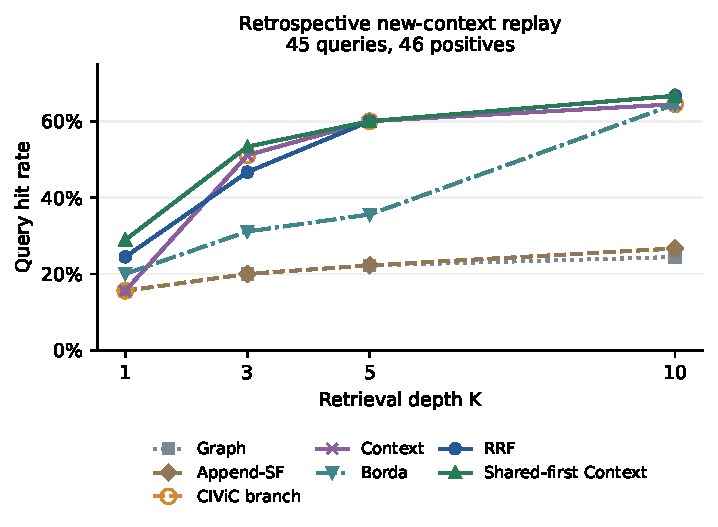
\includegraphics[width=.96\textwidth]{generated/replay_hr_at_k_with_context.pdf}
\caption{Hit rates}
\label{fig:hrk}
\end{figure}


The CIViC-only comparison changes support as well as order. Its replay MRR is 0.3452, with 27/45 hits at five. The single extra covered positive under RRF is dasatinib for MP:6050 at rank 28; it contributes at most $1/(45\cdot28)=0.0008$ query MRR. Most of the $+0.0444$ difference therefore concerns already accessible positives, but the paired intervals still span zero.

\paragraph{Conditional source order.}
Table~\ref{tab:order-ablation} adds graph-order permutations to the archived clinical-order experiment. Replay graph shuffling lowers mean MRR by 0.0462 and HR@3 by 9.07 percentage points. Its MRR upper-tail $p=0.0324$ becomes 0.2915 after the specified 12-test Holm correction. Clinical shuffling lowers mean replay HR@5 by 9.15 points; 17/5,000 draws match or exceed the observed 27 hits, giving $p=18/5001=0.0036$ and Holm $p=0.0432$. Only that comparison survives 0.05 across the family. Development graph MRR exceeds its central 95\% upper quantile, but its Holm $p=0.0550$.
% Generated from frozen artifacts; edit build_revision_tables.py, not numeric cells.
\begin{table}[t]
\centering
\caption{Order shuffles}
\label{tab:order-ablation}
\small
\setlength{\tabcolsep}{2.2pt}
\begin{tabular}{llrrrrr}
\toprule
Shuffled & Metric & Observed & Mean & Central 95\% & Upper $p$ & Holm $p$ \\
\midrule
Graph & MRR & 0.3895 & 0.3433 & $[\,0.2974,\,0.3929\,]$ & 0.0324 & 0.2915 \\
Graph & HR@3 (\%) & 46.67 & 37.59 & $[\,31.11,\,44.44\,]$ & 0.0074 & 0.0740 \\
Graph & HR@5 (\%) & 60.00 & 57.07 & $[\,53.33,\,60.00\,]$ & 0.2044 & 1.0000 \\
CIViC & MRR & 0.3895 & 0.3514 & $[\,0.3085,\,0.3969\,]$ & 0.0498 & 0.3983 \\
CIViC & HR@3 (\%) & 46.67 & 42.82 & $[\,35.56,\,48.89\,]$ & 0.2134 & 1.0000 \\
CIViC & HR@5 (\%) & 60.00 & 50.85 & $[\,46.67,\,55.56\,]$ & 0.0036 & 0.0432 \\
\bottomrule
\end{tabular}
\end{table}


Membership and the unshuffled branch's complete order remain fixed, including the clinical SF terminal key. Accordingly, these perturbations quantify conditional order sensitivity, not removal of all information from either source. The replay graph lists have median length 30 (range 0--50; one empty), and clinical lists median eight (0--36; two empty). Empty branches remain in the denominator; full distributions and all 12 comparisons are retained in S1.

\subsection{Limits under two fixed source orders}
\begin{table}[t]
\caption{Interleaving results}
\label{tab:oracle}
\centering\small
\begin{tabularx}{\textwidth}{@{}l@{\hspace{6pt}}X@{\hspace{5pt}}r@{}}
\toprule
Policy & Ordering constraint & MRR$_q$ \\
\midrule
Append-SF & $O$ followed by $N_{\mathrm{SF}}$ & 0.2004 \\
Append-CIViC & $O$ followed by $N_e$ & 0.2018 \\
Original insertion & Fixed $O,N_v$, $\lambda=4$ & 0.2064 \\
Evidence insertion & Fixed $O,N_e$, $\lambda=4$ & 0.2065 \\
Two-sequence oracle & Best merge of $O,N_e$ & 0.3294 \\
RRF & Full $L_g,L_e$ fusion & 0.3895 \\
Old-order oracle & Fixed $O$, freely ordered additions & 0.4568 \\
\bottomrule
\end{tabularx}
\end{table}
Changing the append suffix from SF to CIViC order barely changes MRR; both yield ten top-five hits (Table~\ref{tab:oracle}). The two insertion policies also yield ten hits. At the development-selected penalty, both retain all old top-five positives and place none of the 13 evidence-exclusive positives in the top five.

The best label-informed merge of fixed $O,N_e$ reaches at most 0.3294 MRR under Eq.~\eqref{eq:bound}, below RRF's 0.3895. These label-informed oracles are explanatory ceilings, not deployable rankings. Exceeding the two-sequence ceiling implies relaxing at least one of the two specified within-sequence constraints. It does not imply that the graph order must change: preserving only that order and freely reordering additions raises the ceiling to 0.4568.

% Generated from frozen artifacts; edit build_revision_tables.py, not numeric cells.
\begin{table}[t]
\centering
\caption{Case study}
\label{tab:cases}
\small
\setlength{\tabcolsep}{2pt}
\begin{tabular}{llrrrrr}
\toprule
Query context & Drug & App. & Alt. & Ctx. & Shared & RRF \\
\midrule
Jan. Breast MP:263 & dovitinib & 41 & 41 & 1 & 4 & 5 \\
Jan. Breast MP:263 & erdafitinib & 33 & 6 & 40 & 40 & 41 \\
W1 Colorectal MP:5117 & pembrolizumab & 7 & 7 & 1 & 1 & 2 \\
W1 Midline glioma MP:3807 & dordaviprone & 14 & 14 & 1 & 1 & 1 \\
W3 Melanoma MP:281$^*$ & belvarafenib & -- & -- & -- & -- & -- \\
\bottomrule
\end{tabular}
\end{table}

The original five case-study rows are retained with the new controls (Table~\ref{tab:cases}), where App., Alt., Ctx. and Shared denote Append-SF, AltAppend, Context and Shared-first Context. A dash marks an unretrieved positive; the asterisk identifies cutoff-defined belvarafenib, outside the 45-query replay. For January breast MP:263, RRF moves evidence-exclusive dovitinib from rank 41 under Append-SF to five, while Context already puts it first. Graph-exclusive erdafitinib moves from 33 to 41 under RRF. In replay, Context and Shared-first already place pembrolizumab and dordaviprone first; fusion is not required for those successes. The unretrieved cutoff-defined belvarafenib remains a negative case.

Provenance describes the cross-context links without validating treatment efficacy. Of 27 RRF top-five replay positives, 13 have cutoff benefit evidence for the exact profile in another or unspecified disease, while 14 share a gene with the evidence profile. For example, level-B dordaviprone evidence for glioma MP:2289 links to MP:3807 through H3-3A.

\subsection{Dependence and parameter sensitivity}
\label{sec:rq4}
The earlier development RRF--AltAppend analysis uses 17 drug and 18 source components, with $+0.0448$ MRR and intervals $[+0.0102,+0.1099]$ and $[+0.0108,+0.1095]$ (S1). It concerns a different cohort and weaker comparator than the replay Context comparison. Removing development's 14 entrectinib pairs leaves 27 queries and 29 pairs: RRF reaches 0.2142, Append-SF 0.1772 and AltAppend 0.1658; Context can exceed RRF on that subset.

Across 54 fusion settings, RRF's replay MRR always exceeds Append-SF's but improves on Context in only part of the grid. The settings vary $k\in\{10,20,40,60,80,100\}$ and graph weight $\alpha\in\{.1,.2,\ldots,.9\}$. All exceed both Context and CIViC on development MRR. In replay, only 30/54 exceed either strong baseline and 24 fall below; no MRR ties occur. HR@5 has 24 settings above, six tied and 24 below both baselines. In the nine-setting neighborhood $k\in\{40,60,80\}$, $\alpha\in\{.4,.5,.6\}$, replay hits range from 19 to 30 of 45. Thus the all-setting advantage over Append-SF does not establish robustness against stronger baselines; the default remains frozen.

\subsection{Source sensitivity and temporal scope}
% Generated from frozen artifacts; edit build_revision_tables.py, not numeric cells.
\begin{table}[t]
\centering
\caption{Source exclusion}
\label{tab:source-exclusion}
\small
\setlength{\tabcolsep}{3.5pt}
\begin{tabular}{lrrrrr}
\toprule
Policy & MRR$_q$ & Pair cov. & HR@1 & HR@3 & HR@5 \\
\midrule
RRF & 0.3330 & 26/39 & 7/39 & 16/39 & 22/39 \\
Context & 0.2924 & 26/39 & 3/39 & 19/39 & 23/39 \\
CIViC & 0.2915 & 25/39 & 3/39 & 19/39 & 23/39 \\
\bottomrule
\end{tabular}
\end{table}

Linking the evidence actually used at cutoff to frozen label supports identifies overlap for 7/46 replay pairs (15.22\%), affecting six queries. The audit covers 11,171 used-evidence rows and 46 eligible positive-label support rows, with no missing source IDs. These are used-evidence intersections, not occurrences anywhere in the snapshot or only among successful hits.

Removing those labels leaves 39 queries and 39 pairs at unchanged ranks (Table~\ref{tab:source-exclusion}). RRF retains MRR differences of $+0.0406$ from Context and $+0.0415$ from CIViC, but hits one fewer query at five than either. This is descriptive sensitivity: the same publication may support distinct contexts, and neither overlap nor its removal resolves every form of leakage or dependence.

The union covers 14/17, 6/6 and 13/23 replay pairs in W1--W3. It misses 13/46 overall, including ten in W3; no union-ranking policy can retrieve those missing pairs. In the separate three-query cutoff-defined cohort, RRF ranks W1 selpercatinib first and misses both W3 belvarafenib positives. The sealed September--October pilot contains two eligible positives and zero hard cases, below its prespecified minima of ten and three; both positives are unretrieved. These small counts and the retrospective main query construction do not establish prospective generalization.

\section{Discussion and Limitations}
\label{sec:discussion}
The central result is the gap between an improvement over appending and an established advantage over competitive same-pool ordering. RRF's replay MRR point estimate exceeds Context's, but both cluster intervals span zero. Shared-first Context attains a higher replay point estimate, with the ordering reversed in development. Favoring shared candidates can therefore reproduce and exceed the observed replay gain without establishing its causal source, a new default, or a statistically superior policy. Neither an interval crossing zero nor a reversal across these small cohorts establishes equivalence or ineffectiveness.

Retrieval depth and positive-level retention expose different trade-offs. Equal query HR@5 can mask which evidence-exclusive positives are promoted and which old hits are retained. The permutations condition on fixed memberships and the other branch's complete order, including the SF terminal key in the clinical list. Only replay clinical HR@5 survives the specified 12-test Holm correction; the graph results do not justify either universal benefits or an absence of graph information. Likewise, exceeding the two-sequence ceiling requires relaxing at least one specified order constraint, not necessarily the graph order.

Source overlap further limits interpretation. Removing confirmed overlapping labels leaves 39 queries and 39 pairs at unchanged ranks. RRF retains a positive MRR difference from Context but hits one fewer query at five. Shared publications can support distinct contexts, so overlap does not automatically invalidate a label; stability after exclusion cannot certify that all leakage or dependence has been removed.

These are post hoc diagnostics of a small, single-knowledgebase retrospective replay. CIViC curation shapes both visible evidence and the endpoint; unlabeled relevance remains unknown. The three cutoff-defined queries and separate underpowered pilot do not establish prospective generalization. The results concern annotation retrieval, not clinical efficacy.

\section{Conclusion}
EvidencePath makes candidate access, shared membership, and conditional source ordering separately inspectable. Frozen-score expansion can increase coverage while lowering MRR, and a simple shared-first control can exceed RRF's replay point estimate. Paired uncertainty, retrieval-depth trade-offs, provenance sensitivity, and specified-sequence bounds delimit these observations rather than establish a universally superior fusion policy.

\begin{thebibliography}{99}
\bibitem{primekg}
Chandak, P., Huang, K., Zitnik, M.: Building a knowledge graph to enable precision medicine. Sci. Data \textbf{10}, 67 (2023). \url{https://doi.org/10.1038/s41597-023-01960-3}
\bibitem{civic2022}
Krysiak, K., et al.: CIViCdb 2022: evolution of an open-access cancer variant interpretation knowledgebase. Nucleic Acids Res. \textbf{51}(D1), D1230--D1241 (2023). \url{https://doi.org/10.1093/nar/gkac979}
\bibitem{rrf}
Cormack, G.V., Clarke, C.L.A., Buettcher, S.: Reciprocal rank fusion outperforms Condorcet and individual rank learning methods. In: SIGIR, pp. 758--759 (2009). \url{https://doi.org/10.1145/1571941.1572114}
\bibitem{pushpakom}
Pushpakom, S., et al.: Drug repurposing: progress, challenges and recommendations. Nat. Rev. Drug Discov. \textbf{18}, 41--58 (2019). \url{https://doi.org/10.1038/nrd.2018.168}
\bibitem{txgnn}
Huang, K., et al.: A foundation model for clinician-centered drug repurposing. Nat. Med. \textbf{30}, 3601--3613 (2024). \url{https://doi.org/10.1038/s41591-024-03233-x}
\bibitem{aurora}
Zhang, Y., Duan, L., Zheng, H., Xu, J.: AURORA: An adaptive multi-granularity graph learning framework for drug repositioning. In: DASFAA 2026. LNCS, vol. 16537, pp. 149--164. Springer (2026). \url{https://doi.org/10.1007/978-981-92-0369-7_10}
\bibitem{civic}
Griffith, M., et al.: CIViC is a community knowledgebase for expert crowdsourcing the clinical interpretation of variants in cancer. Nat. Genet. \textbf{49}, 170--174 (2017). \url{https://doi.org/10.1038/ng.3774}
\bibitem{civiccuration}
Danos, A.M., et al.: Standard operating procedure for curation and clinical interpretation of variants in cancer. Genome Med. \textbf{11}, 76 (2019). \url{https://doi.org/10.1186/s13073-019-0687-x}
\bibitem{civicmp}
CIViC: Molecular Profiles Overview. \url{https://docs.civicdb.org/en/latest/model/molecular_profiles/overview.html} (accessed 7 November 2026)
\bibitem{oncokb}
Chakravarty, D., et al.: OncoKB: a precision oncology knowledge base. JCO Precis. Oncol. \textbf{1}, 1--16 (2017). \url{https://doi.org/10.1200/PO.17.00011}
\bibitem{escat}
Mateo, J., et al.: A framework to rank genomic alterations as targets for cancer precision medicine: the ESMO Scale for Clinical Actionability of molecular Targets (ESCAT). Ann. Oncol. \textbf{29}(9), 1895--1902 (2018). \url{https://doi.org/10.1093/annonc/mdy263}
\bibitem{genedrug}
Su, L., Xie, X., Qian, W., Shao, M., He, Y., Zhang, L.: GeneDrug: A retrieval platform for analyzing gene-drug relations in cancer. In: DASFAA 2026. LNCS, vol. 16540, pp. 699--702. Springer (2026). \url{https://doi.org/10.1007/978-981-92-0378-9_50}
\bibitem{ggef}
Su, L., Xie, X., Qian, W., Li, M., Ma, S., Shao, M., Zhang, L.: GGEF: A framework for automatic extraction of gene-drug relationships from cancer guidelines. In: DASFAA 2026. LNCS, vol. 16540, pp. 186--199. Springer (2026). \url{https://doi.org/10.1007/978-981-92-0378-9_12}
\bibitem{pandrugs2}
Jim\'enez-Santos, M.J., et al.: PanDrugs2: prioritizing cancer therapies using integrated individual multi-omics data. Nucleic Acids Res. \textbf{51}(W1), W411--W418 (2023). \url{https://doi.org/10.1093/nar/gkad412}
\bibitem{lambdamart}
Burges, C.J.C.: From RankNet to LambdaRank to LambdaMART: an overview. Microsoft Research Technical Report MSR-TR-2010-82 (2010)
\bibitem{lightgbm}
Ke, G., et al.: LightGBM: a highly efficient gradient boosting decision tree. In: Advances in Neural Information Processing Systems, vol. 30, pp. 3146--3154 (2017)
\bibitem{metasearch}
Aslam, J.A., Montague, M.: Models for metasearch. In: SIGIR, pp. 276--284 (2001). \url{https://doi.org/10.1145/383952.384007}
\bibitem{bruch}
Bruch, S., Gai, S., Ingber, A.: An analysis of fusion functions for hybrid retrieval. ACM Trans. Inf. Syst. \textbf{42}(1), Article 20 (2024). \url{https://doi.org/10.1145/3596512}
\bibitem{cawley}
Cawley, G.C., Talbot, N.L.C.: On over-fitting in model selection and subsequent selection bias in performance evaluation. J. Mach. Learn. Res. \textbf{11}, 2079--2107 (2010)
\bibitem{kapoor}
Kapoor, S., Narayanan, A.: Leakage and the reproducibility crisis in machine-learning-based science. Patterns \textbf{4}(9), 100804 (2023). \url{https://doi.org/10.1016/j.patter.2023.100804}
\bibitem{exp4fuse}
Liu, L., Zhang, M.: Exp4Fuse: A rank fusion framework for enhanced sparse retrieval using large language model-based query expansion. In: Findings of the Association for Computational Linguistics: ACL 2025, pp. 163--173 (2025). \url{https://doi.org/10.18653/v1/2025.findings-acl.9}
\end{thebibliography}

\end{document}
